%%%%%%%%%%%%%%%%%%%%%%%%%%%%%%%%%%%%

\section{2.4. Variáveis aleatórias}

%%%%%%%%%%%%%%%%%%%%%%%%%%%%%%%%%%%%

\begin{frame}
\frametitle{Variáveis aleatórias}

\begin{itemize}
\justifying
\item Uma \hl{variável aleatória} é uma quantidade numérica cujo valor depende do resultado de um evento aleatório.
\begin{itemize}
\justifying
\item Usamos uma letra maiúscula, como $ X $, para denotar uma variável aleatória.
\justifying
\item Os valores de uma variável aleatória são denotados com uma letra minúscula, neste caso $ x $.
\justifying
\item Por exemplo, $P(X = x)$.
\end{itemize}
\justifying
\item Existem dois tipos de variáveis aleatórias:
\begin{itemize}
\justifying
\item \hl{Variáveis aleatórias discretas} representam valores inteiros.
\begin{itemize}
\justifying
\item Exemplo: Número de filhos, número de carros, número de clientes de uma loja,...
\end{itemize}
\justifying
\item \hl{Variáveis aleatórias contínuas} valores reais
\begin{itemize}
\justifying
\item Exemplo: Preço de um livro, peso, altura, tempo...
\end{itemize}
\end{itemize}

\end{itemize}

\end{frame}

%%%%%%%%%%%%%%%%%%%%%%%%%%%%%%%%%%%%

\subsection{Esperança}

%%%%%%%%%%%%%%%%%%%%%%%%%%%%%%%%%%%%

\begin{frame}
\frametitle{Esperança}

\begin{itemize}
\justifying
\item Estamos frequentemente interessados no resultado médio de uma variável aleatória.
\justifying
\item Chamamos isso de \hl{valor esperado} (média). A média é uma soma ponderada dos possíveis resultados.\\
\formula{\[\mu = E(X) = \sum_{i = 1}^k x_i ~ P(X = x_i)\]}

\end{itemize}

\end{frame}

%%%%%%%%%%%%%%%%%%%%%%%%%%%%%%%%%%%%

\begin{frame}
\frametitle{Valor esperado de uma variável aleatória discreta}
\justifying
\dq{Em um jogo de cartas, você ganha \$ 1 se tirar um coração, \$ 5 se você comprar um ás (incluindo o ás de copas), \$ 10 se você tirar o rei de espadas e nada para qualquer outra carta que você selecionar. Escreva o modelo de probabilidade para seus ganhos e calcule seu ganho esperado.}

\pause

\begin{center}
\scalebox{0.85}{
\renewcommand{\arraystretch}{1.5}
\begin{tabular}{l | c | c | c }
Evento		& $X$ 		& $P(X)$        		& $X ~ P(X)$ \\
\hline
Coração (não de ás)	& $1$		& $\frac{12}{52}$	& $\frac{12}{52}$ \\
Ás			& $5$		& $\frac{4}{52}$	& $\frac{20}{52}$ \\	
Rei de espadas	& $10$		& $\frac{1}{52}$	& $\frac{10}{52}$ \\	
Todos os outros		& $0$		& $\frac{35}{52}$	& $0$ \\
\hline
Total			&			&				& $E(X) = \frac{42}{52} \approx 0.81$
\end{tabular}
}
\end{center}

\end{frame}

%%%%%%%%%%%%%%%%%%%%%%%%%%%%%%%%%%%%

\begin{frame}
\frametitle{Valor esperado de uma variável aleatória discreta (cont.)}
\justifying
Abaixo está uma representação visual da distribuição de probabilidade dos ganhos deste jogo:

\begin{center}
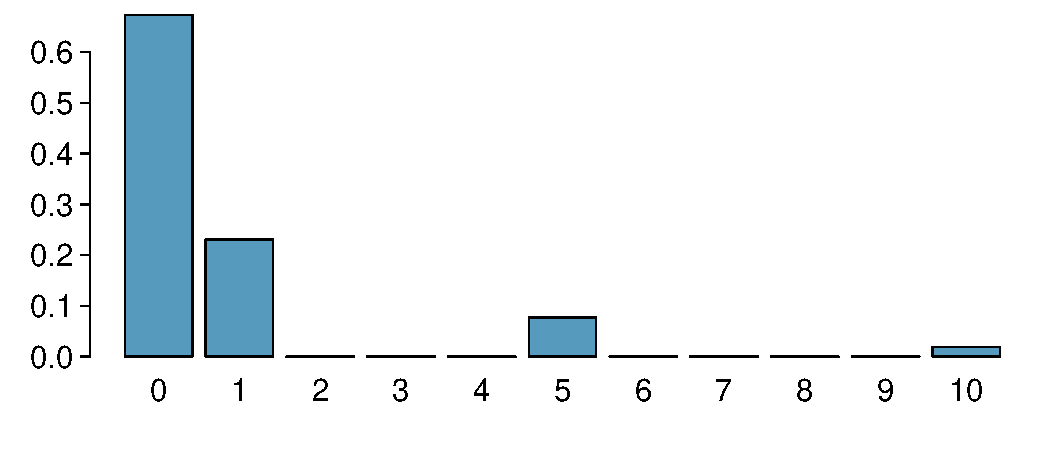
\includegraphics[width=0.8\textwidth]{2-4_random_variables/card_game.pdf}
\end{center}

\end{frame}

%%%%%%%%%%%%%%%%%%%%%%%%%%%%%%%%%%%%

\subsection{Variância de variáveis aleatórias}

%%%%%%%%%%%%%%%%%%%%%%%%%%%%%%%%%%%%

\begin{frame}
\frametitle{Variância}
\justifying
Também estamos frequentemente interessados na variabilidade dos valores de uma variável aleatória.

\formula{
\[ \sigma^2 = Var(X) = \sum_{i = 1}^k (x_i - E(X))^2 P(X = x_i) \]
\[ \sigma = SD(X) = \sqrt{Var(X)} \]
}

\end{frame}

%%%%%%%%%%%%%%%%%%%%%%%%%%%%%%%%%%%%

\begin{frame}
\frametitle{Variância de uma variável aleatória discreta}
\justifying
\dq{Para o exemplo anterior do jogo de cartas, quanto você esperaria que os ganhos variassem de jogo para jogo?}

\vspace{2mm}
\only<2->{

\scalebox{0.75}{
\begin{center}
\renewcommand{\arraystretch}{2}
\begin{tabular}{c | c | c | l | p{4cm}}
$X$ & $P(X)$         & $X ~ P(X)$      & \multicolumn{1}{c|}{$(X - E(X))^2$}  & \multicolumn{1}{c}{$P(X) ~ (X - E(X))^2$}  \\
\hline
1 & $\frac{12}{52}$  & $1 \times \frac{12}{52} = \frac{12}{52}$ & $(1 - 0.81)^2 = 0.0361$ &  $\frac{12}{52} \times 0.0361 = 0.0083$ \\
\hline
5 & $\frac{4}{52}$   & $5 \times \frac{4}{52} = \frac{20}{52}$ & $(5 - 0.81)^2 = 17.5561$  & $\frac{4}{52} \times 17.5561 = 1.3505$ \\
\hline
10  & $\frac{1}{52}$ & $10 \times \frac{1}{52} = \frac{10}{52}$  & $(10 - 0.81)^2 = 84.4561$   & $\frac{1}{52} \times 84.0889 = 1.6242$ \\
\hline
0 & $\frac{35}{52}$  & $0 \times \frac{35}{52} = 0$  & $(0 - 0.81)^2 = 0.6561$ & $\frac{35}{52} \times 0.6561 = 0.4416$ \\
\hline
  &       & $E(X) = 0.81$ & & \soln{\only<3->{$V(X) = 3.4246$}} \\
 &       &                                                         & & \soln{\only<4>{$SD(X) = \sqrt{3.4246} = 1.85$}} \\
\end{tabular}
\end{center}
}
}
\end{frame}

%%%%%%%%%%%%%%%%%%%%%%%%%%%%%%%%%%%%

\subsection{Combinações lineares de variáveis aleatórias}

%%%%%%%%%%%%%%%%%%%%%%%%%%%%%%%%%%%%

\begin{frame}
\frametitle{Combinações lineares}

\begin{itemize}
\justifying
\item Uma \hl {combinação linear} de variáveis aleatórias $ X $ e $ Y $ é dada por\\

\[ aX + bY \]

onde $a$ e $b$ são alguns números fixos.

\pause
\justifying
\item O valor médio de uma combinação linear de variáveis aleatórias é dado por\\
\formula{\[ E(aX + bY) = a \times E(X) + b \times E(Y) \]}

\end{itemize}

\end{frame}

%%%%%%%%%%%%%%%%%%%%%%%%%%%%%%%%%%%%

\begin{frame}
\frametitle{Calculando a esperança de uma combinação linear}
\justifying
\dq{Imagine que em média, você leva 10 minutos para fazer um exercício de estatística e 15 minutos para terminar um exercício de física. Esta semana você deve fazer uma lista com 5 exercícios de estatística e um trabalho com 4 exercícios de física. Qual o tempo total que você espera gastar para fazer as duas tarefas?}\\

\soln{
\pause
\begin{align*} 
E(Est + Est + Est + Est + Est + Fis + Fis + Fis + Fis) &= 5 \times E(Est) + 4 \times E(Fis) \\
&= 5 \times 10 + 4 \times 15 \\
&= 50 + 60 \\
&= 110~min 
\end{align*}
}

\end{frame}

%%%%%%%%%%%%%%%%%%%%%%%%%%%%%%%%%%%%

\subsection{Variância de combinações lineares de variáveis aleatórias}

%%%%%%%%%%%%%%%%%%%%%%%%%%%%%%%%%%%%

\begin{frame}
\frametitle{Combinações lineares}

\begin{itemize}
\justifying
\item A variância de uma combinação linear de duas variáveis aleatórias independentes é\\
\formula{\[ V(aX + bY) = a^2 \times V(X) + b^2 \times V(Y) \]}

\pause 
\justifying
\item O desvio padrão da combinação linear é a raiz quadrada da variância.

\pause 

\justifying
\item Se as variáveis aleatórias não forem independentes, o cálculo da variância fica um pouco mais complicado\\
\formula{\[ V(aX + bY) = a^2 \times V(X) + b^2 \times V(Y) + 2abCov(X, Y) \]}


\end{itemize}

\end{frame}

%%%%%%%%%%%%%%%%%%%%%%%%%%%%%%%%%%%%

\begin{frame}
\frametitle{Calculando a variância de uma combinação linear}
\justifying
\dq{O desvio padrão do tempo que você leva para cada problema de estatística é 1,5 minutos, e é de 2 minutos para cada problema de física. Qual é o desvio padrão do tempo que você espera gastar? Suponha que o tempo para resolver cada exercício seja independente do outro.}\\

\soln{
\pause
\small{
\begin{align*} 
V(Est + Est + Est + Est + Est + Fis + Fis + Fis + Fis) &= V(Est) + V(Est) + V(Est) + V(Est) + V(Est)  \\
& + V(Fis) + V(Fis) + V(Fis) + V(Fis) \\
&= 5 \times V(Est) + 4 \times V(Fis) \\
&= 5 \times 1.5^2 + 4 \times 2^2 \\
&= 27.25
\end{align*}
}}

\end{frame}

%%%%%%%%%%%%%%%%%%%%%%%%%%%%%%%%%%%%

\subsection{Relembrando}

%%%%%%%%%%%%%%%%%%%%%%%%%%%%%%%%%%%%

\begin{frame}
\frametitle{Prática}
\justifying
\pq{Um jogo de cartas em um cassino custa \$5 por partida. Se a primeira carta que você tirar for vermelha, você poderá comprar uma segunda carta (sem substituição). Se a segunda carta é o ás de paus, você ganha \$500. Se não, você não ganha nada, ou seja, perde os \$5. Qual é o lucro/prejuízo esperado ao jogar este jogo? {\small Lembre-se: lucro/perda = ganhos - custo.}}


\begin{multicols}{2}
\begin{enumerate}[(a)]
\item Um lucro de 5\$
\solnMult{Uma perda de 10\$}
\item Uma perda de 25\$
\item Uma perda de 30\$
\end{enumerate}
\end{multicols}

\vspace{-1cm}



\begin{table}[!h]\footnotesize
\scriptsize
\centering
\begin{tabular}{l c c c r}
Evento				& Ganho	& Lucro: $X$	& $P(X)$	& $ X \times P(X)$	\\
\hline
\orange{Vermelho}, {A}{$\clubsuit$}		& 500		& 500 - 5 = 495	& $\frac{26}{52} \times \frac{1}{51} = 	0.0098$ & 	 $495 \times 0.0098 = 4.851$ \\
Outros	& 0 			& 0 - 5 = -5	& $1 - 0.0098 = 0.9902$ & $-5 \times 0.9902 = -4.951$ \\  
\hline
					&			&			& 			& $E(X) = -0.1$
\end{tabular}
\end{table}


\end{frame}

%%%%%%%%%%%%%%%%%%%%%%%%%%%%%%%%%%%%

\begin{frame}
\frametitle{Jogo Justo}
\justifying
Um jogo \hl{justo} é definido como um jogo em que o custo e o prêmio esperado são iguais, ou seja, o lucro esperado é 0.

\pause

$\:$
\justifying
\dq{Você acha que os jogos nos cassinos em Vegas custam mais ou menos do que os ganhos esperados?}

\soln{
\pause
\begin{columns}[c]
\column{0.6\textwidth}
\justifying
Se esses jogos custassem menos do que o esperado, isso significaria que em médias os cassinos perderiam dinheiro:
\column{0.4\textwidth}
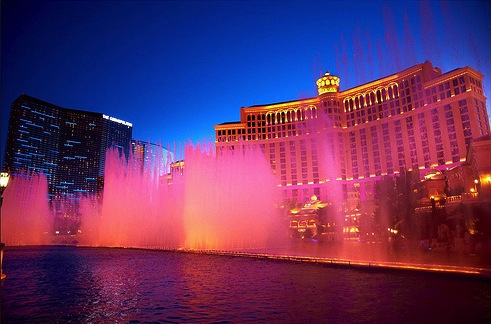
\includegraphics[width=\textwidth]{2-4_random_variables/bellagio.jpg}
\end{columns}
\ct{Image by Moyan\_Brenn on Flickr \webURL{http://www.flickr.com/photos/aigle\_dore/5951714693}.}
}


\end{frame}

%%%%%%%%%%%%%%%%%%%%%%%%%%%%%%%%%%%%%

\begin{frame}
\frametitle{Propriedades de Variáveis Aleatórias}
\justifying
Variáveis aleatórias não funcionam como variáveis algébricas:\\
\[ X + X \ne 2X \]

\pause

{\small
\twocol{0.45}{0.45}
{
\begin{align*}
E(X + X) &= E(X) + E(X) \\
&= 2 E(X) \\
&~  \\
E(2X) &= 2 E(X) \\
&~ 
\end{align*}
}
{
\begin{align*}
Var(X + X) &= Var(X) + Var(X)~{\scriptsize \text{(assumindo independência)}} \\
&= 2~Var(X) \\
&~  \\
Var(2X) &= 2^2~Var(X) \\
&= 4~Var(X)
\end{align*}
}
}


\pause

\vspace{3mm}

\mathhl{E(X + X)  = E(2X)}, mas \mathhl{Var(X + X) \ne Var(2X)}.

\end{frame}

%%%%%%%%%%%%%%%%%%%%%%%%%%%%%%%%%%%%%

\begin{frame}
\frametitle{Adicionando ou multiplicando?}
\justifying
\dq{Uma empresa tem 5 carros em sua frota, aados históricos mostram que o custo anual de manutenção para cada carro é, em média, de \$ 2.154 com um desvio padrão de \$ 132. Qual é a média e o desvio padrão do custo total anual de manutenção para esta frota ?}

\pause
\justifying
Note que temos 5 carros, cada um com custo anual de manutenção $(X_1 + X_2 + X_3 + X_4 + X_5)$.

\pause
\end{frame}
%%%%%%%%%%%%%%%%%%%%%%%%%%%%%%%%%%%%%

\begin{frame}
\frametitle{Adicionando ou multiplicando?}

\scalefont{0.8}
\begin{eqnarray*} 

E(X_1 + X_2 + X_3 + X_4 + X_5) &=& E(X_1) + E(X_2) + E(X_3) + E(X_4) + E(X_5) \\
\pause

&=& 5 \times E(X) = 5 \times 2,154 = \$ 10,770 \\
\pause

Var(X_1 + X_2 + X_3 + X_4 + X_5) &=& Var(X_1) + Var(X_2) + Var(X_3) + Var(X_4) + Var(X_5) \\
\pause

&=& 5 \times V(X) = 5 \times 132^2 = \$ 87,120 \\
\pause

SD(X_1 + X_2 + X_3 + X_4 + X_5) &=& \sqrt{87,120} =  295.16

\end{eqnarray*}


\end{frame}
%%%%%%%%%%%%%%%%%%%%%%%%
